\documentclass[12pt]{article}

\usepackage{amsmath,amsthm,amsfonts,amssymb,amsxtra}
\usepackage{pgf,tikz}
\usetikzlibrary{arrows}
\renewcommand{\theenumi}{(\alph{enumi})} 
\renewcommand{\labelenumi}{\theenumi}

\pagestyle{empty}
\setlength{\textwidth}{7in}
\setlength{\oddsidemargin}{-0.5in}
\setlength{\topmargin}{-1.0in}
\setlength{\textheight}{9.5in}

\newtheorem{problem}{Problem}

\begin{document}

\noindent{\large\bf MATH 242}\hfill{\large\bf Third Midterm.}\hfill{\large\bf
  Spring 2012}\hfill{\large\bf Page 1/5}\hrule

\bigskip
\begin{center}
  \begin{tabular}{|ll|}
    \hline & \cr
    {\bf Name: } & \makebox[12cm]{\hrulefill}\cr & \cr
    {\bf 4-digit code:} & \makebox[12cm]{\hrulefill}\cr & \cr
    \hline
  \end{tabular}
\end{center}
\begin{itemize}
\item Write your name and the last 4 digits of your SSN in the space provided above.
\item The test has five (5) pages, including this one and the table of
  Laplace transforms at the end.
\item Show sufficient work to justify all answers unless otherwise
  stated in the problem.  Correct answers with inconsistent work may
  not be given credit. 
\item Credit for each problem is given at the right of each problem
  number. 
\item No books, notes or calculators may be used on this test.
\end{itemize}
\hrule

\begin{center}
  \begin{tabular}{|c|c|c|}
    \hline
    &&\cr
    {\large\bf Page} & {\large\bf Max} & {\large\bf Points} \cr
    &&\cr
    \hline
    &&\cr
    {\Large 2} & \Large 35 & \cr
    &&\cr
    \hline
    &&\cr
    {\Large 3} & \Large 30 & \cr
    &&\cr
    \hline
    &&\cr
    {\Large 4} & \Large 35 & \cr
    &&\cr
    \hline\hline
    &&\cr
    {\large\bf Total} & \Large 100 & \cr
    &&\cr
    \hline
  \end{tabular}
\end{center}
\newpage

%%%%%%%%%%%%%%%%%%%%%%%%%%%%%%%%%%%%% Page 2
\noindent{\large\bf MATH 242}\hfill{\large\bf Third Midterm.}\hfill{\large\bf
  Spring 2012}\hfill{\large\bf Page 2/5}\hrule

\bigskip
{\problem[20 pts] \em Use exclusively techniques based on the Laplace
  transform to solve the initial value problem $x''+3x'+2x=t$ that
  satisfies $x(0)=0, x'(0)=2$.} 
\vspace{14cm}
\begin{flushright}
  \begin{tikzpicture}
    \draw (0cm,-0.2cm) rectangle (5cm,1.2cm);
  \end{tikzpicture}
\end{flushright}
\hrule
{\problem[15pts] \em Find the Laplace transform of $f(x) = \sin 3x
  \cos 3x.$}
\vspace{4cm}
\begin{flushright}
  \begin{tikzpicture}
    \draw (0cm,-0.2cm) rectangle (5cm,1.2cm);
  \end{tikzpicture}
\end{flushright}

\newpage
%%%%%%%%%%%%%%%%%%%%%%%%%%%%%%%%%%%%% Page 3
\noindent{\large\bf MATH 242}\hfill{\large\bf Third Midterm.}\hfill{\large\bf
  Spring 2012}\hfill{\large\bf Page 3/5}\hrule

\bigskip
{\problem[20 pts] \em Use exclusively the technique of variation of
  parameters to solve the differential equation $y''+3y'+2y=x$.}
\vspace{14cm}
\begin{flushright}
  \begin{tikzpicture}
    \draw (0cm,-0.2cm) rectangle (5cm,1.2cm);
  \end{tikzpicture}
\end{flushright}
\hrule
{\problem[10pts] \em Find the Laplace transform of $f(x)=\sin(x)/x.$}
\vspace{4cm}
\begin{flushright}
  \begin{tikzpicture}
    \draw (0cm,-0.2cm) rectangle (5cm,1.2cm);
  \end{tikzpicture}
\end{flushright}
\newpage

%%%%%%%%%%%%%%%%%%%%%%%%%%%%%%%%%%%%% Page 4
\noindent{\large\bf MATH 242}\hfill{\large\bf Third Midterm.}\hfill{\large\bf
  Spring 2012}\hfill{\large\bf Page 4/5}\hrule

\bigskip
{\problem[15 pts] \em Use exclusively the method of undetermined
  coefficients to solve the differential equation $\frac{d^2
    f}{d\omega^2}(\omega) + 3\frac{df}{d\omega}(\omega) + 2f(\omega) =
  \omega.$}
\vspace{6cm}
\begin{flushright}
  \begin{tikzpicture}
    \draw (0cm,-0.2cm) rectangle (5cm,1.2cm);
  \end{tikzpicture}
\end{flushright}
\hrule
{\problem[20] \em Find the inverse Laplace transform of
  $F(s)=(s^2+b^2)^{-2}$}
\vspace{11.5cm}
\begin{flushright}
  \begin{tikzpicture}
    \draw (0cm,-0.2cm) rectangle (5cm,1.2cm);
  \end{tikzpicture}
\end{flushright}
\newpage

%%%%%%%%%%%%%%%%%%%%%%%%%%%%%%%%%%%%% Page 5
\noindent{\large\bf MATH 242}\hfill{\large\bf Third Midterm.}\hfill{\large\bf
  Spring 2012}\hfill{\large\bf Page 5/5}\hrule

\bigskip
\begin{center}
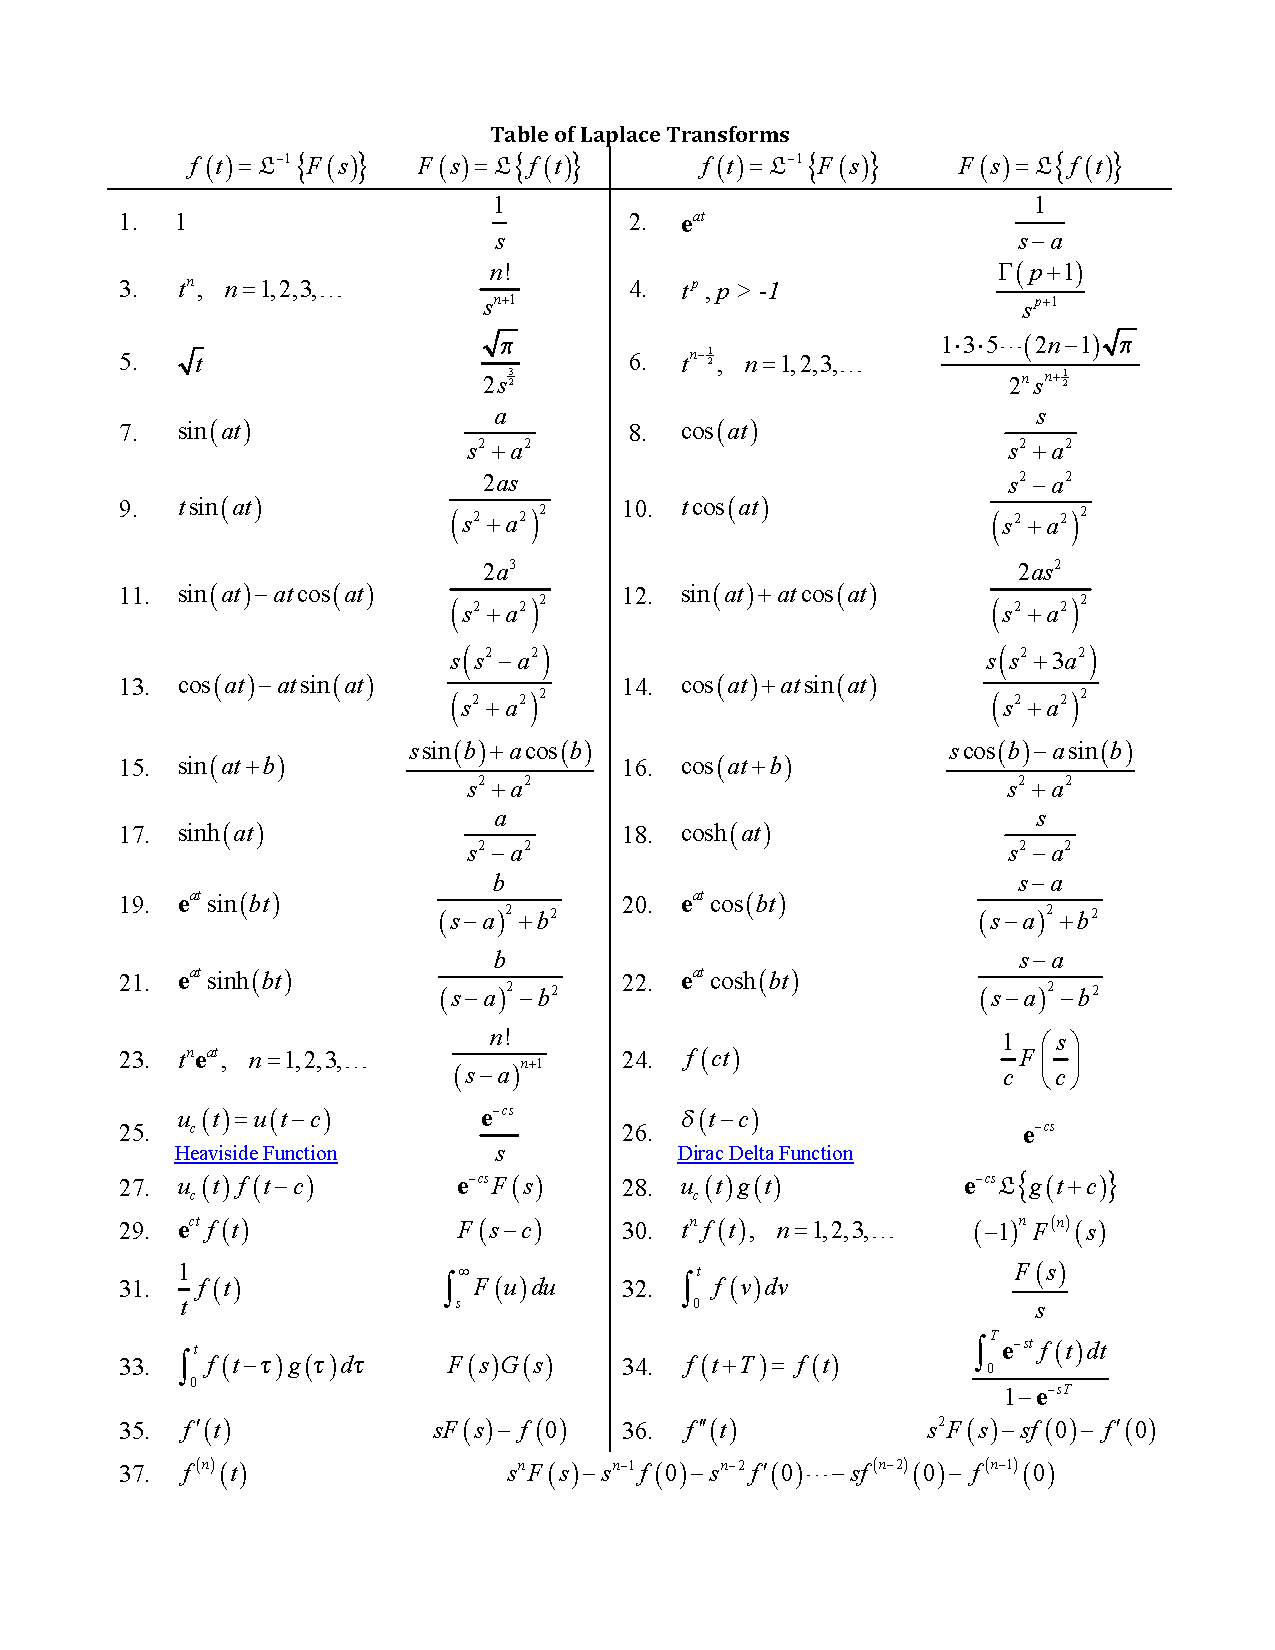
\includegraphics[width=0.7\linewidth]{table.pdf}
\end{center}


\end{document}
